%!TEX root = ../main.tex
\section{Three Phase Inverter}
\label{sec:inverter}
This section will describe the design of the three phase inverter used to drive the PMAC motor in this project.
This includes the calculations and considerations done.
Initially, a short overview of the principle of operation of a three phase inverter is given.

\subsection{Operation of a Three Phase Inverter}
A three phase inverter enables the use of a DC supply in variable frequency control of a three phase load.
In this project the DC supply is a battery and the load, a PMAC motor.
Figure \ref{fig:threephaseinverter} is a Simulink model showing the most basic three phase inverter.
As can be seen, the inverter consists of three half-bridges for a total of six switches.
Each pair of switches can never be on at the same time as this would result in shorting the battery.

\begin{figure}[!h]
	\centering
	\includegraphics[width=\linewidth,trim=0cm 5cm 0cm 1cm]{graphics/threephaseinverter}
	\caption{Simulink model of a simple three phase inverter for a balanced load.}
	\label{fig:threephaseinverter}
\end{figure}

This type of inverter only works with a balanced load, such as the PMAC motor.
A balanced three phase load implies, that the sum of the currents in the three phases is always equal tp zero, and no current is running through a neutral wire.
As the inverter does not have a connection to the neutral point of the load, it could not supply an unbalanced load, such as those in uninterruptible power supplies (UPS's) and solar cells.

Several schemes exist to control the switches.
Throughout this project a PWM modulation technique using sinusoids as reference is used.
Figure \ref{fig:countercarrier} is a depiction of the modulation technique.
A carrier wave is compared to a sinusoidal reference signal.
By low-pass filtering the output voltage, the fundamental frequency can be revealed.
Whenever the reference crosses the carrier wave, the gate voltages of the relevant half-bridge invert, of course the necessary dead time has to be added to avoid short circuiting the power rail.
This technique produces naturally sampled, center aligned PWM, a desirable trait due to the lower harmonic distortion when compared to other types of PWM.

\begin{figure}[h!]
	\centering
	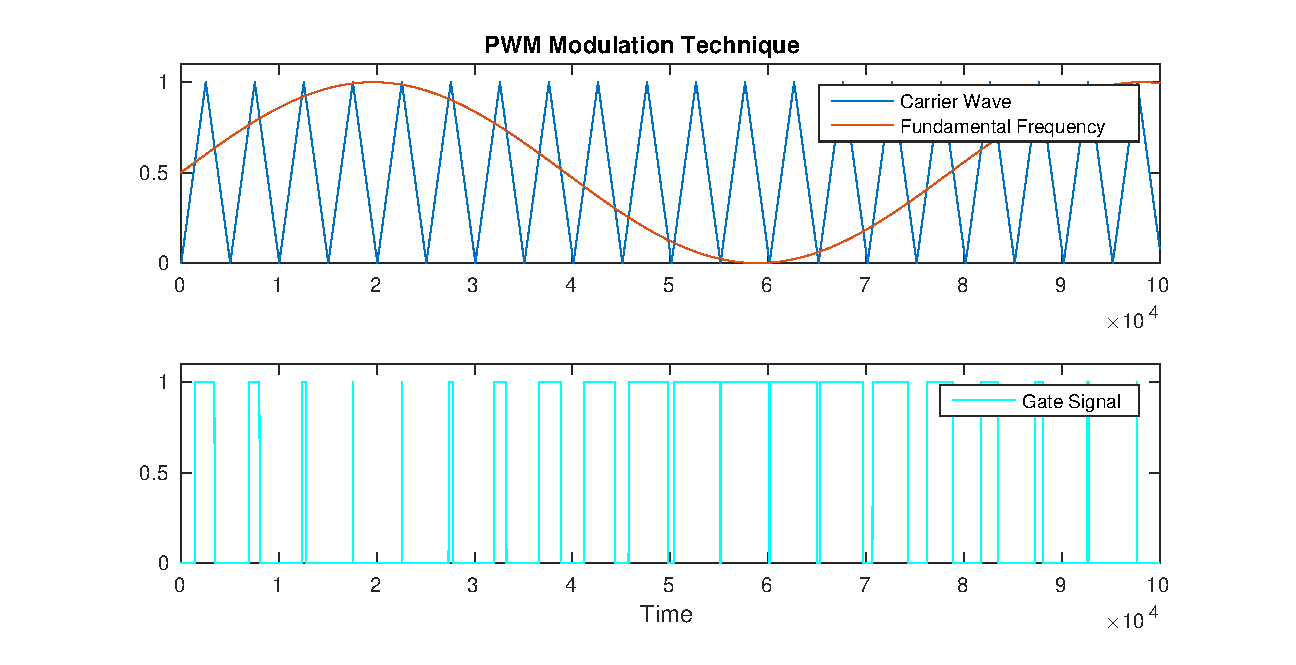
\includegraphics[width=\linewidth]{graphics/countercarrier}
	\caption{Naturally sampled PWM using a sinusoid as fundamental frequency.}
	\label{fig:countercarrier}
\end{figure}

\subsection{Choosing the MOSFETs}\label{sub:choosing_mosfets}
\label{sec:mosfet}
Before choosing MOSFETs for the three phase inverter one will have to keep in mind the application parameters.
Firstly, the batteries\cite{superB} will have an average nominal voltage of $52.8$\si{\volt} and end of charge voltage at $60.8\si{\volt}$.
The MOSFETs will therefor need to be able to handle a minimum drain to source voltage, $V_{DS}$, of 60.8\si{\volt}. 
Secondly, the current drawn by the motor can reach a maximum peak of 300A.
Thirdly, the motor driver\cite{DRV8301} will supply a gate voltage, $V_{GS}$, of 9.5\si{\volt} to 11.5\si{\volt}. 
The MOSFETs will therefore need to be fully conducting at $V_{GS} = 9.5V$ and be able to handle the driver supplied range.
The three main requirements are listed in table \ref{tab:req1}\\

\begin{table}[h!]
	\centering
	\begin{tabular}{clr}
		  & Requirement\\
		  \hline
		1 & Can handle minimum voltage of & 60.8\si{\volt}\\
		2 & Can handle minimum current of & 300\si{\ampere}\\
		3 & Operating at $V_{GS}$ of  & 9.5\si{\volt} \\
		\hline
	\end{tabular}
	\caption{Three main requirements as a starting point for choosing the MOSFETs.}
	\label{tab:req1}
\end{table}

Due to high currents through the MOSFETs, the heat dissipation is assumed to be high as well. 
To prevent overheating and burning out the MOSFETs they will be mounted on to a heat sink. 
Therefore a through hole package will be required for this application. 
Because of its size and easy mounting, the chosen package is the TO-247 \cite{TO_247}. 
The TO-247 is the largest housing available and is not capable of handling the current.
When looking for MOSFETs that add up to the requirements of table~\ref{tab:req1}, the International rectifier power MOSFET IRFP4468PBF is chosen.
It does not exactly meet the requirements, but paralleling at least two of these will.

\begin{table}[h!]
	\centering
\begin{tabular}{|l|l|c|c|c|c|}
	\hline
\rowcolor[HTML]{C0C0C0}	\multicolumn{1}{|c|}{Symbol} & \multicolumn{1}{|c|}{Parameter} & Min. & Typ. &
	 Max. & Units\\
	\hline
	$I_D$ & Continuous Drain Current (Silicon Limited) & - & - & 290 &  \multirow{2}{*}{A}\\
	\cline{1-5}
	%\multirow{3}{*}{\si{\celsius/W}}\\
	%\cline{1-3}
	$I_D$ & Continuous Drain Current (Package Limited) & - & - & 195 &\\
	\hline
	$V_{GS}$ & Gate to Source Voltage & - & - & $\pm$20 & \multirow{3}{*}{V}\\
	\cline{1-5}
	 $V_{GS(th)}$ & Gate Threshold Voltage & 2.0 & - & 4.0 & \\
	 \cline{1-5}
	 $V_{(BR)DSS}$ & Drain to Source Breakdown Voltage & 100 & - & - & \\
	 \hline
	 $R_{DS(on)}$ & Static Drain to Source On Resistance & - & 2.0 & 2.6 & m$\Omega$\\
	 \hline
	 
\end{tabular}
\caption{Some important parameters from the IRFP4468PBF MOSFET datasheet\cite{IRF4468PbF}. All parameters are found at junction temperature $T_J = 25^{\circ}$C.}
\label{tab:MOSdata}
\end{table}
The TO-247 package has a continuous drain current limit of 195A that is only around two third of the minimum current requirement. 
With that in mind, the MOSFET parameters in table~\ref{tab:MOSdata} seem to be a  suitable choice for the application if more than one MOSFET is used for each switching side. 
Using a parallel setup, the MOSFETs are assumed to share the current equally. 
If one would draw more current than the others, the temperature would rise causing $R_{DS(on)}$ to rise as seen in figure~\ref{fig:tj_rds}. 
Which will result in reduced current.
As will be later discussed, parallel setup will also have an effect on the total power loss.


\subsection{Power Loss}

The total power loss, $P_{loss}$ of a switching device can be estimated using equation~\ref{eq:p_loss} where $P_c$ and $P_{sw}$ are conduction- and switching losses respectively.  

\begin{equation}
P_{loss} = P_{c} + P_{sw}
\label{eq:p_loss}
\end{equation}

For simplicity the power loss will be estimated from a single phase of the inverter circuit seen in figure~\ref{fig:single_phase}. 
The current $I_{out}$ is drawn by some load $R_{load}$ that will absorb the load power $P_{load}$ which is given by equation \ref{eq:p_load}. 
Since there are two switches, $Q_1$ and $Q_2$, it is assumed that the load power is delivered equally from both. The output power, $P_{Q}$, of each switch is given by equation~\ref{eq:P_Q}  


\begin{figure}[!h]
	\centering
	\includestandalone[width=0.2\textwidth]{graphics/mosfets}
	\caption{Single phase from where the MOSFET current is calculated.}
	\label{fig:single_phase}
\end{figure}


\begin{equation}
P_{load} = R_{load} I_{out,RMS}^2
\label{eq:p_load}
\end{equation}

\begin{equation}
P_{Qi} = \dfrac{P_{load}}{2} = R_{load} I_{Qi,RMS}^2
\label{eq:P_Q}
\end{equation}


Inserting equation~\ref{eq:p_load} into~\ref{eq:P_Q} and solving for $I_{Qi,RMS}$, equation~\ref{eq:I_qRMS} is formed.

\begin{equation}
\dfrac{R_{load} I_{out,RMS}^2}{2} = R_{load} I_{Qi,RMS}^2 \rightarrow I_{Qi,RMS} = \dfrac{I_{out,RMS}}{\sqrt{2}} 
\label{eq:I_qRMS}
\end{equation}
Which then again can be expressed as in equation~\ref{eq:I_qi}.

\begin{equation}
I_{Qi,RMS} = \dfrac{I_{out,RMS}}{\sqrt{2}} = \dfrac{I_{out}}{\sqrt{2}\sqrt{2}} = \dfrac{I_{out}}{2}
\label{eq:I_qi}
\end{equation}


As mentioned earlier each switching setup will consist of $n$ number of MOSFETs in parallel. 
Therefore the drain current of each parallel MOSFET becomes $I_{Pi,RMS}$ in equation~\ref{eq:I_pi}.

\begin{equation}
I_{Pi,RMS}=\dfrac{I_{Qi,RMS}}{n} = \dfrac{I_{out}}{2n}
\label{eq:I_pi}
\end{equation}

\subsubsection{Conduction loss}\label{sub:Cunduction_loss}


Conduction loss of each MOSFET can be calculated using equation~\ref{eq:p_c}

\begin{equation}
P_{c} = R_{DS(on)}\cdot I_{Pi,RMS}^2
\label{eq:p_c}
\end{equation}


Although listed in the datasheet, the drain to source resistance $R_{DS(on)}$ only applies to the  $T_J = 25 \si{\celsius}$ condition. 
The resistance will vary with the junction temperature $T_J$. 
The relation between $T_J$ and $R_{DS(on)}$ can be seen in figure~\ref{fig:tj_rds} from where the multiplication factor $\alpha$ in equation~\ref{eq:Rdstj} can be estimated.

\begin{equation}
R_{DS(on),@T_J} =  \alpha R_{DS(on),@25\si{\celsius}}
\label{eq:Rdstj}
\end{equation}

\begin{figure}[h!]
	\centering
	\includegraphics[scale =0.7]{graphics/T_n_R_compare}
	\caption{The $R_{DS(on)}$ and $T_J$ relation at $I_D = 180A$ and $V_{GS} = 10V$\cite{IRF4468PbF}.}
	\label{fig:tj_rds}
\end{figure}

If assumed that the junction temperature will be around $100 \si{\celsius}$ one can estimate the factor being approximately $\alpha = 1.6$. 
The instantaneous conduction loss for each MOSFET in parallel can then be estimated using equations~\ref{eq:p_c}, \ref{eq:I_pi} and \ref{eq:Rdstj} to form equation~\ref{eq:P_cp}.

\begin{equation}
P_{c} = R_{DS(on),@100\si{\celsius}} I_{Pi,RMS}^2 =  R_{DS(on),@100\si{\celsius}} \bigg(\dfrac{I_{out}}{2n}\bigg)^2
\label{eq:P_cp}
\end{equation}

\subsubsection{Switching Loss}
Whenever any MOSFET is switching from its on state to its off state or vice versa, a small amount of energy is lost, as the MOSFET passes through its active region.
This loss can be found with experiments or estimated from calculations. 
An experiment will not be carried out at this point but the loss will be estimated with calculations and assumptions using equation~\ref{eq:P_sw}.

\begin{equation}
P_{sw} = \dfrac{1}{2} V_{in} I_D (t_{c,on} + t_{c,off} ) f_{s}
\label{eq:P_sw}
\end{equation}

where $I_D$ is the drain current, $I_{Pi,RMS}$, of each MOSFET from equation~\ref{eq:I_pi} and $\mathrm{V_{in}}$ is the supply voltage for the inverter. 
The times $t_{c,on} $ and $ t_{c,off} $ are the combined on and off time respectively and are defined in figure~\ref{fig:sw_loss} as equation~\ref{eq:time_on} and~\ref{eq:time_off}

\begin{figure}[h!]
	\centering
	\includegraphics[scale = 0.5]{graphics/sw_losses}
	\caption[MOSFET switching losses.]{MOSFET switching losses. $t_{ri}$ and $t_{fi}$ are the current,$I_D$, rise and fall times respectively and $t_{rv}$ and $t_{fv}$ are the rise and fall time of $D_{DS}$ respectively\cite{pwrElectronics}.}
	\label{fig:sw_loss}
\end{figure}

\begin{eqnarray}
t_{c,on} = t_{ri} + t_{fv}
\label{eq:time_on}\\
t_{c,off} = t_{rv} + t_{fi}
\label{eq:time_off}
\end{eqnarray}

The voltage rise and fall times, $t_{rv}$ and $t_{fv}$ respectively, in figure~\ref{fig:sw_loss} are the time it takes the drain to source voltage, $V_{DS}$ to rise from zero to $V_{in}$ and opposite. 
The values are defined in the MOSFET datasheet\cite{IRF4468PbF} as the rise and fall times $t_r$ and $t_f$ seen in figure~\ref{fig:sw_time_wavef}. 
The times are listed in table~\ref{tab:tf_tr}.
Equation~\ref{eq:tfv_tr} and \ref{eq:trv_tf} show the relation.

\begin{figure}[h!]
	\centering
	\includegraphics[scale = 0.5]{graphics/sw_time_wavef}
	\caption{Switching Time Waveforms\cite{IRF4468PbF}.}
	\label{fig:sw_time_wavef}
\end{figure}

\begin{table}[h!]
	\centering
	\begin{tabular}{|c|c|c|c|}
		\hline
\rowcolor[HTML]{C0C0C0}		Symbol & Parameter & Typ. & Units\\
		\hline
		$t_r$ & Rise Time & 230 & \multirow{2}{*}{ns}\\
		$t_f$ & Fall Time & 260 & \\
		\hline
	\end{tabular}
	\caption{$V_{GS}$ rise and fall time taken from datasheet\cite{IRF4468PbF}.}
	\label{tab:tf_tr}
\end{table}


\begin{eqnarray}
t_{fv} = t_r\label{eq:tfv_tr}\\
t_{rv} = t_f\label{eq:trv_tf}
\end{eqnarray}

The turn on and off characteristics of the MOSFETs are shown in figure~\ref{fig:turn_on_off}. 
From there one can see that the current rise and fall times, $t_{ri}$ and $t_{fi}$ respectively, are the same times as it takes the gate voltage $V_{GS}$ to rise from $V_{GS(th)}$ to $V_{GS(I_0)}$ for the on state and opposite for the off state.



\begin{figure}[h!]
	\centering
	\begin{subfigure}[b]{0.4\textwidth}
		\includegraphics[width=\textwidth]{graphics/mos_turn_on}
		\caption{Turn on characteristic.}
		\label{fig:Turn_on}
	\end{subfigure}
	~
	\begin{subfigure}[b]{0.4\textwidth}
		\includegraphics[width=\textwidth]{graphics/mos_turn_off}
		\caption{Turn off characteristic.}
		\label{fig:Turn_off}
	\end{subfigure}
	\caption{The turn on and off characteristics of the MOSFETs\cite{pwrElectronics}.}
	\label{fig:turn_on_off}
\end{figure}

The gate to source current, $I_{gs}$ is defined in equation \ref{eq:I_gs} where $dt$ is the current rise and fall times $t_{ri}$ and $t_{fi}$ respectively. 
$dV$ is the difference between $V_{GS(th)}$ and $V_{GS(I_0)}$ as seen in equation~\ref{eq:dv} and $n$ is the number of MOSFETs in parallel.

\begin{equation}
I_{gs} = nC\dfrac{dV}{dt} 
\label{eq:I_gs}
\end{equation}

\begin{equation}
dV = |V_{GS(I_0)} - V_{GS(th)}|
\label{eq:dv}
\end{equation}

For simplicity it is assumed that the gate charge current remains constant. 
Then one can assume that the gate to source current is known. 
The motor driver sources up to $1.7\si{\ampere}$ when switching to the on state and sinks up to $2.3\si{\ampere}$ when switching to the off state\cite{DRV8301}. 
Equation~\ref{eq:I_gs} can then be rearranged for $dt$ as shown in equation~\ref{eq:dt}. 
It is assumed that the charge current will be constant for the duration of the turn on and turn off times.

\begin{equation}
dt = nC\dfrac{dV}{I_{gs}}
\label{eq:dt}
\end{equation}



\subsection{Total Power Loss}

The instantaneous power losses are calculated for up to 10 MOSFETs in parallel using equations~\ref{eq:P_cp}, \ref{eq:P_sw} and~\ref{eq:p_loss} where the switching frequency is $f_s = 20\si{\kilo\hertz}$. Figures~\ref{fig:ploss_single} and~\ref{fig:ploss_comb} shows the results.


\begin{figure}[h!]
	\centering
	\includegraphics[scale = 0.5]{graphics/pwr_loss_single}
	\caption{Instantaneous power losses of a single MOSFET in a parallel setup as a function of number of MOSFETs.}
	\label{fig:ploss_single}
\end{figure}

In figure~\ref{fig:ploss_single} the losses are calculated for each MOSFET in a parallel setup of $n$ MOSFETs. 
One will notice, as previously stated, that the number of MOSFETs in parallel, affects the power losses significantly.
The conduction loss will decrease rapidly and will become close to nothing when $n$ increases. 
This happens because the current is equally divided between the MOSFETs, thus, each MOSFET has less current flowing through. 
The switching loss however increases with $n$ and will become dominant. In that case the gate capacitance will increase by a factor of $n$ causing the switching loss to increase.

\begin{figure}[h!]
	\centering
	\includegraphics[scale = 0.5]{graphics/pwr_loss_comb}
	\caption{Combined instantaneous power losses of each parallel setup as a function of number of MOSFETs.}
	\label{fig:ploss_comb}
\end{figure}

From the combined power loss shown in figure~\ref{fig:ploss_comb}, it is clear that the total instantaneous power loss is smallest when $n = 2$ or $P_{loss} \approx 95\si{\watt}$. 
The design will have two MOSFETs in parallel switching each phase. The average power loss at maximum RMS current will become for all three phases as seen in equation~\ref{eq:P_loss_total}.
\begin{equation}
P_{loss,total} = 95\cdot 6 = 570\si{\watt}
\label{eq:P_loss_total}
\end{equation}

\subsection{Temperature}

The power losses defined in previous sections will cause the MOSFETs to heat up while operating. 
Therefore they will be mounted onto a heat sink as mentioned in section \ref{sub:choosing_mosfets}. 
To get an estimate on how hot the MOSFETs will be, equations~\ref{eq:Ta}, \ref{eq:Tc} and \ref{eq:Tj} are used. 
$T_s$ is the heat sink temperature, $T_c$ the case temperature  and $T_j$ is the junction temperature.
The parameters can be seen in table~\ref{tab:temp_param}. 
To get an estimate of the temperature it is assumed that the time it takes the go-kart to get from zero to full speed, $t = 5s$. 
The system will for that time be operating at maximum torque, for maximum time.
In reality, other factors will effect the power dissipation but will not be discussed further.
 

\begin{table}[h!]
	\centering
	\begin{tabular}{|c|l|c|c|}
		\hline
\rowcolor[HTML]{C0C0C0}		Symbol & \multicolumn{1}{c|}{Parameter} & Value & Units\\
		\hline
		$T_{J,max}$ & MOSFET maximum junction temperature & 175 & \si{\celsius}\\
		\hline
		$R_{jc}$ & MOSFET junction to case thermal resistance & 0.29 & \multirow{3}{*}{\si{\celsius/W}}\\
		\cline{1-3}
		$Re_{cs}$ & MOSFET case to sink thermal resistance & 0.24 &\\
		\cline{1-3}
		$R_{sa}$ & Heat sink thermal resistance & 0.29 & \\
		\hline
		$C_s$ & Heat sink thermal capacitance  & 2190 &\si{\joule/\celsius}\\
		\hline
		$P_{loss,total}$ & Instantaneous power loss of each MOSFET & 570 & \si{\watt}\\
		\hline
	\end{tabular}
	\caption{Parameters used to calculate the temperature.}
	\label{tab:temp_param}
\end{table}



\begin{eqnarray}
T_s  & = & (R_{sa}P_{loss,total})\bigg(1-exp(-\dfrac{t}{R_{sa}C_s})\bigg) + T_a
\label{eq:Ta}\\
T_c & = & T_s + P_{loss}R_{cs}
\label{eq:Tc}\\
T_j & = & T_c + P_{loss}R_{jc}
\label{eq:Tj}
\end{eqnarray}

The temperatures are calculated to be:

\begin{eqnarray*}
T_s & = &  26\si{\celsius}\\
T_c & = &  49\si{\celsius}\\
T_j & = &  77\si{\celsius}\\
\end{eqnarray*}

The calculated junction temperature is well below the maximum ratings shown in table~\ref{tab:temp_param}. If it is assumed that the go-kart will be operating with full power loss for t = 5min the temperature will reach $T_j \approx$ 140\si{\celsius}. Thus, it is safe to assume that the MOSFETs will not reach the maximum limit.


\subsection{Inverter Layout}
The layout of the inverter was mostly done by the other group though discussion about design and assembly were made between the two groups.
In this section the overall principles of the layout is described.
As the inverter has to switch large currents, all parasitic inductances should be avoided.
This is generally done by avoiding long wires as they all contribute with extra inductance.
Wires are not completely avoidable, but they should be kept short, and forward and return wires should be twisted to keep them in close proximity.\\
The power stage of the inverter needs a higly conductive ground plane as well as a power plane, which is connected to the battery voltage.
This is done with two 1mm thick plates of copper, separated by Kapton tape. 
This is a temperature resistant insulating tape meaning that there is no galvanic connection from the power plane on top, to the ground plane on the bottom.
The developed layout can be seen in figure \ref{fig:inverter_design}.

\begin{figure}[h!]
	\centering
	\includegraphics[width=0.7\linewidth]{graphics/Bertha1}
	\caption{Picture of the finished three phase inverter with mounted Zybo, analogue and digital boards.}
	\label{fig:inverter_design}
\end{figure}

As it can be seen, the the inverter was build on a large heat sink, along with the the Zybo, digital and analogue boards. 
This heat sink is much larger than needed, but it was chosen for its structural integrity along with its cooling capability.
The heat sink is mounted on an aluminium box, that blocks for air flow from the sides.\\
Below the heat sink three fans were places to produce airflow on the heat sink for better heat dissipation.
This was necessary because the heat sink needs to be mounted vertically for passive convection to work properly. \\ 

The wires from the batteries will introduce inductance to the system in the order of a few \si{\micro\henry}.
This will cause the current not to change instantaneously, when the upper MOSFETs are switched.
Capacitors are added to filter this behavior.
It is chosen to add eight Panasonic Aluminum Electrolytic Capacitors , each having capacitance of 2200$\mu$F.
Those are added to smoothen out low frequency voltage spikes.
These each have an equivalent series resistance of 57\si{\milli\ohm}, and can handle currents of 4.06\si{\ampere} each.
To counter for the higher frequency, another eight film capacitors with capacitance of 4.7$\mu$F are added.
  
